\subsection{Jaollisuus ja luvun tekijät}

\luettelolaatikko{Jaollisuus}{
	§ \textbf{Määritelmä $1$.} Kokonaisluku $a$ on \termi{jaollisuus}{jaollinen} kokonaisluvulla $b \neq 0$, jos on olemassa kokonaisluku $c$ niin, että $a = b \cdot c$. Tällöin sanotaan myös, että $b$ on $a$:n \termi{tekijä}{tekijä}. Voidaan merkitä $b \mid a$, joka luetaan ''$b$ jakaa $a$:n'' tai ''$b$ on $a$:n tekijä''.

	\vspace*{24pt}

	§ \textbf{Määritelmä $2$.} Luku $a$ on jaollinen luvulla $b \neq 0$, mikäli $\frac{a}{b}$ on kokonaisluku.
	Määritelmät ovat yhtäpitäviä.
}

Jaollisuudesta puhutaan vain käsiteltäessä kokonaislukuja (eli siis myös luonnollisia lukuja) -- käsite ei yleisty mielekkäästi rationaali- tai reaaliluvuille.

\begin{esimerkki}
	\alakohdat{
		§ Luku $-12$ on jaollinen luvulla $3$, sillä $-12 = 3 \cdot (-4)$.
		§ $-12$ ei ole jaollinen luvulla $5$, sillä ei ole kokonaislukua, joka kerrottuna viidellä olisi $12$.
	}
\end{esimerkki}

\begin{esimerkki}
	\alakohdat{
		§ Väite $4\mid12$ on tosi.
		§ Väite $4\nmid 5$ on tosi.
	}
\end{esimerkki} 
   
%\begin{center}
%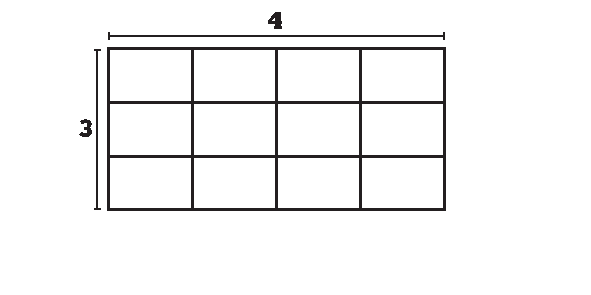
\includegraphics[scale=0.85]{pictures/Kuva2-4-3x4.pdf}
%\end{center}
    
Kaikki luvut ovat jaollisia itsellään ja luvulla $1$.

\begin{esimerkki}
\alakohdat{
§ $7=7 \cdot 1=1 \cdot 7$, joten $7$ on jaollinen luvuilla $1$ ja $7$, koska sekä $1$ että $7$ ovat kokonaislukuja.
§ $-6=-6 \cdot 1=1 \cdot (-6)$, joten $-6$ on jaollinen sekä itsellään että yhdellä.
}
\end{esimerkki}

Kokonaislukuja, jotka ovat jaollisia kahdella, sanotaan \termi{parillinen luku}{parillisiksi luvuiksi}. Lukut, jotka eivät ole parillisia, ovat \termi{pariton luku}{parittomia lukuja}. 

%esim

Jaollisuus on tärkeä käsite lukuteoriassa, ja joidenkin laskutoimitusten ymmärtämisessä, mutta jaollisuuden käsitettä käytetään myös monissa virallisissa määritelmissä nimellisesti matematiikan ulkopuolella. Esimerkiksi vuosi määritellään karkausvuodeksi, jos vuosiluku on jaollinen neljällä mutta ei sadalla, mutta kuitenkin neljälläsadalla jaolliset ovat myös karkausvuosia. Karkausvuonna helmikuu on vuorokauden tavallista pidempi.

%esim

\subsection{Alkuluvut}

\laatikko[Alkuluku]{
	\termi{alkuluku}{Alkuluku} on lukua yksi suurempi luonnollinen luku, joka ei ole jaollinen muilla positiivisilla kokonaisluvuilla kuin luvulla $1$ ja itsellään.
}

\begin{esimerkki}
	\alakohdat{
		§ Luvut $2$, $3$, $5$, $7$, $11$, $13$, $17$ ja $19$ ovat alkulukuja. Tämä voidaan tarkistaa jakamalla kukin luku sitä pienemmillä alkuluvuilla ja toteamalla, että mikään jakolasku ei mene tasan.
		§ Luku $18$ ei ole alkuluku, koska se on jaollinen esimerkiksi luvulla $9$.
		§ Mikään negatiivinen luku ei voi olla alkuluku, koska jokainen negatiivinen luku $-a$ voidaan kirjoittaa tulona $-1\cdot a$.
	}
\end{esimerkki}

Jos luvun tekijä on alkuluku, sitä kutsutaan \termi{alkutekijä}{alkutekijäksi}.

% \begin{esimerkki}
% 	\alakohdat{
% 		§ 
% 	
% 	}
% \end{esimerkki}

\laatikko[Aritmetiikan peruslause]{
Jokainen ykköstä suurempi kokonaisluku voidaan esittää (termien järjestystä lukuunottamatta) yksikäsitteisesti alkulukujen tulona. Jokainen yhtä suurempi kokonaisluku voidaan jakaa alkutekijöihin (termien järjestystä lukuunottamatta) yksikäsitteisellä tavalla.
}

Aritmetiikan peruslause todistetaan kurssilla Logiikka ja lukuteoria. %FIXME: kurssiviittaus

\begin{esimerkki}
Luku $84$ voidaan kirjoittaa muodossa $2\cdot 2\cdot 3\cdot 7$. Havaitaan, että $2$, $3$, ja $7$ ovat kaikki alkulukuja. Aritmetiikan peruslauseen nojalla tiedetään, että tämä on ainoa tapa kirjoittaa $84$ alkulukujen tulona -- mahdollista kerrottavien termien järjestyksen vaihtoa lukuunottamatta.
\end{esimerkki}

Luvun alkutekijät voi löytää etsimällä luvulle ensin jonkin esityksen kahden luvun tulona. Näiden kahden luvun ei tarvitse olla alkulukuja. Sen jälkeen sama toistetaan näille kahdelle luvulle ja edelleen aina uusille luvuille, kunnes jäljellä on vain alkulukuja.

% \begin{esimerkki}
% 	\alakohdat{
% 		§ 
% 	
% 	}
% \end{esimerkki}